\chapter{Introduction}
\section{Motivation}
Since the introduction of Bitcoin, a peer-to-peer payment network and cryptocurrency, there has been countless new cryptocurrencies that is used and traded. Along with this the high volatility has piqued a lot of retail investors interest with some investors gaining a high return of interest and others losing a lot of money~\cite{losing_money_on_crypto_2021}. In addition to this, larger investment institutions have also sought to gain profits from this new type of tradable asset~\cite{gondek_what_nodate}. This has lead there to be more sophisticated forms of cryptocurrency trading.
\\[5mm]
However, trading cryptocurrencies was initially very difficult for people without technical know-how, and the first recorded transaction was on $12^{th}$ October 2009 via a paypal transaction~\cite{noauthor_history_nodate}. Since then, there has been countless other cryptocurrency exchanges have emerged. Many of which are centralized, which provide a simple interface and support for investors with little technical know-how, and others are decentralised, which work by directly interacting with the blockchain. Centralized exchanges are predominantly used as we can see in Figure \ref{fig:dex_to_cex}, however we can also see that the volume traded in DEXes have been increasing since 2020. 

\begin{figure}[htb!]
    \centering
    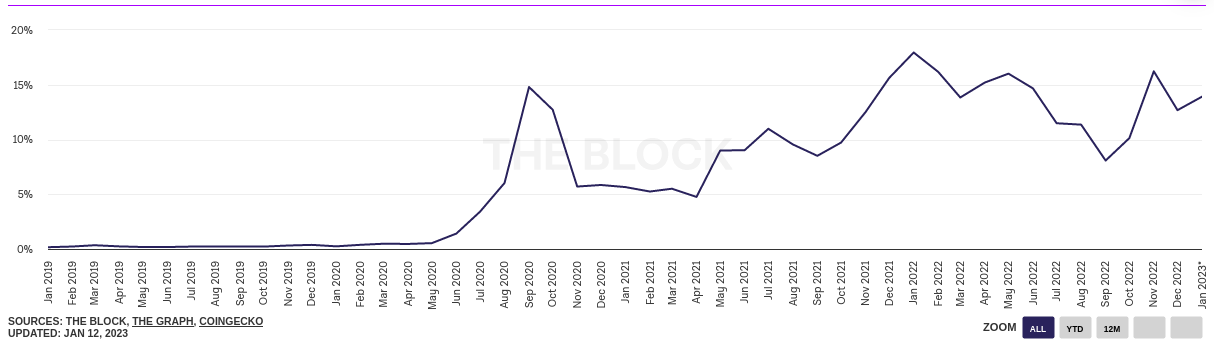
\includegraphics[width=\textwidth]{introduction/Images/dex_to_cex.png}
    \caption{{DEX} to {CEX} {Spot} {Trade} {Volume}~\cite{dex_to_cex}}
    \label{fig:dex_to_cex}
\end{figure}

This poses the question that about which trading strategies can exploit arbitrage opportunities on decentralised exchanges. There has been some research on this topic, mainly focussing on triangular and cyclic arbitrage on DEXes such as Uniswap and SushiSwap, however there has been no research into analysing the performance of statistical arbitrage methods on decentralised exchanges.

\section{Objectives}
\begin{itemize}
    \item Impelement Statistical arbitrage techiniques on Decentralised exchnages
    \item \begin{itemize}
        \item What is Stat Arbitrage
        \item Give an Example
    \end{itemize}
    \item Analyse results
\end{itemize}

\section{Challenges}
\begin{itemize}
    \item Shorting
    \item Smart Contracts
    \item 
\end{itemize}

\section{Contributions}
\begin{itemize}
    \item First ever research on stat. arb on crypto pairs on dex
\end{itemize}